
\documentclass[12pt]{article}
\usepackage[utf8]{inputenc}
\usepackage[T1]{fontenc}
\usepackage{amsmath,amssymb,amsthm} % matematik
\usepackage{natbib}
\usepackage{titlesec}
\usepackage{setspace}
\usepackage{graphicx} % Allows including images

\title{Social Data Science exam project}
\author{Group 9, Rasmus Gars, Lukas Hidan, Hjortur Hjartar and Mads Wulff}
\date{October 2015}


\makeatletter
\renewcommand\thesection{}
\renewcommand\thesubsection{}
\makeatother

\usepackage{caption}
\usepackage{subcaption}

\DeclareCaptionFormat{subfig}{\figurename~#1#2#3}
\DeclareCaptionSubType*{figure}
\captionsetup[subfigure]{format=subfig,labelsep=colon,labelformat=simple}



%\setlength\parindent{0pt}
\onehalfspacing
\usepackage[top=1.5in, bottom=1.5in, left=1in, right=1in]{geometry}
\usepackage{fancyhdr}

\begin{document}
\maketitle

	\section{Purpose} % (fold)
	\label{sec:problem_1}
	In this paper we examine a controversial subject - is the movie better than the book? By collecting and examining user-generated ratings of books and movies, we find that....

	However, there are also several important caveats when examining the data, which we discuss in the paper. 

	Normalisation 



\section{Data} % (fold)
	\label{sec:data}

There are The data collection is subject to a selection bias, which we will discuss later.

\subsection{Movie ratings}
We collect data on movies from the site IMDb.com, which collects a variety of information  of 3,5572,200 titles (including TV-shows, documentaries, etc.) at the time of scraping on December 6th 2015. We collect data on a subset of the entire moviedatabase, namely those who are tagged as "based on novel". This amounts to 20,665 individual films. There are also tv-series and tv-films that are based on movies, but we do not include them.

We are especially interested in the rating of the movies, which is given on a scale of 1 to 10. We also collect the movie title and the number of votes given to the rating. There are some legal issues surrounding the collections of data, that we will discuss later.

IMDb states that their movies ratings are not pure arithmetic means of the ratings. They state that they make some adjustements in order to battle "vote stuffing", ie. inflating votes by rating several times through a computer farm in the Philippines. IMDb does not disclose the method they use to adjust the ratings in order to prevent abuse of it. We use the IMDb rating as it stated on a movie's page, as we believe it is more representative of the average IMDB user than the pure arithmetic mean.

All movies we collect data on are made after the book is published, such that there are no books made on movies. 

\subsection{Book ratings} % (fold)
\label{sub:book_ratings}
We collect data on books from the user-driven site Goodreads, which collects user-generated reviews on novels

We collect the user-generated rating which is given on a scale of 1 to 5. The rating is an arithmetic average of We also collect the book title and the number of votes given in the rating. 


\subsection{Merging book and movie data}
We merge the two data sets

This merging assumes that the title of the book and the movie are the same, which might not be the case. The different naming of books and movies can be made of artistic reasons or to avoid confusion or even trademark issues from other movies. As we merge a subset of movies and films that are stated as being based on books, we assume that the probability of a film not refering to the book of the same insignificant. Some books foster more than one movie based on it. We assume that due to naming and trademark rights, that movies with the same title are based on the same book.


Both subsets of the data are generated by users of the sites and may be subject to false data, unsincere ratings or outright trolling. Both sites have dedicated users, such that we hope that any false data is quickly deleted. 

As referred to above, the IMDb rating is not an arithemtic average, but the Goodreads rating is. We assume that Goodrads also make some effort to battle "vote stuffing"

\subsection{Making book and movie data comparable}

\section{Discussion} % (fold)
\label{sec:discussion}

% section discussion (end)

\subsection{Number of votes cast}

\begin{figure}[!ht]
  \begin{subfigure}[b]{.5\linewidth}
    \centering
    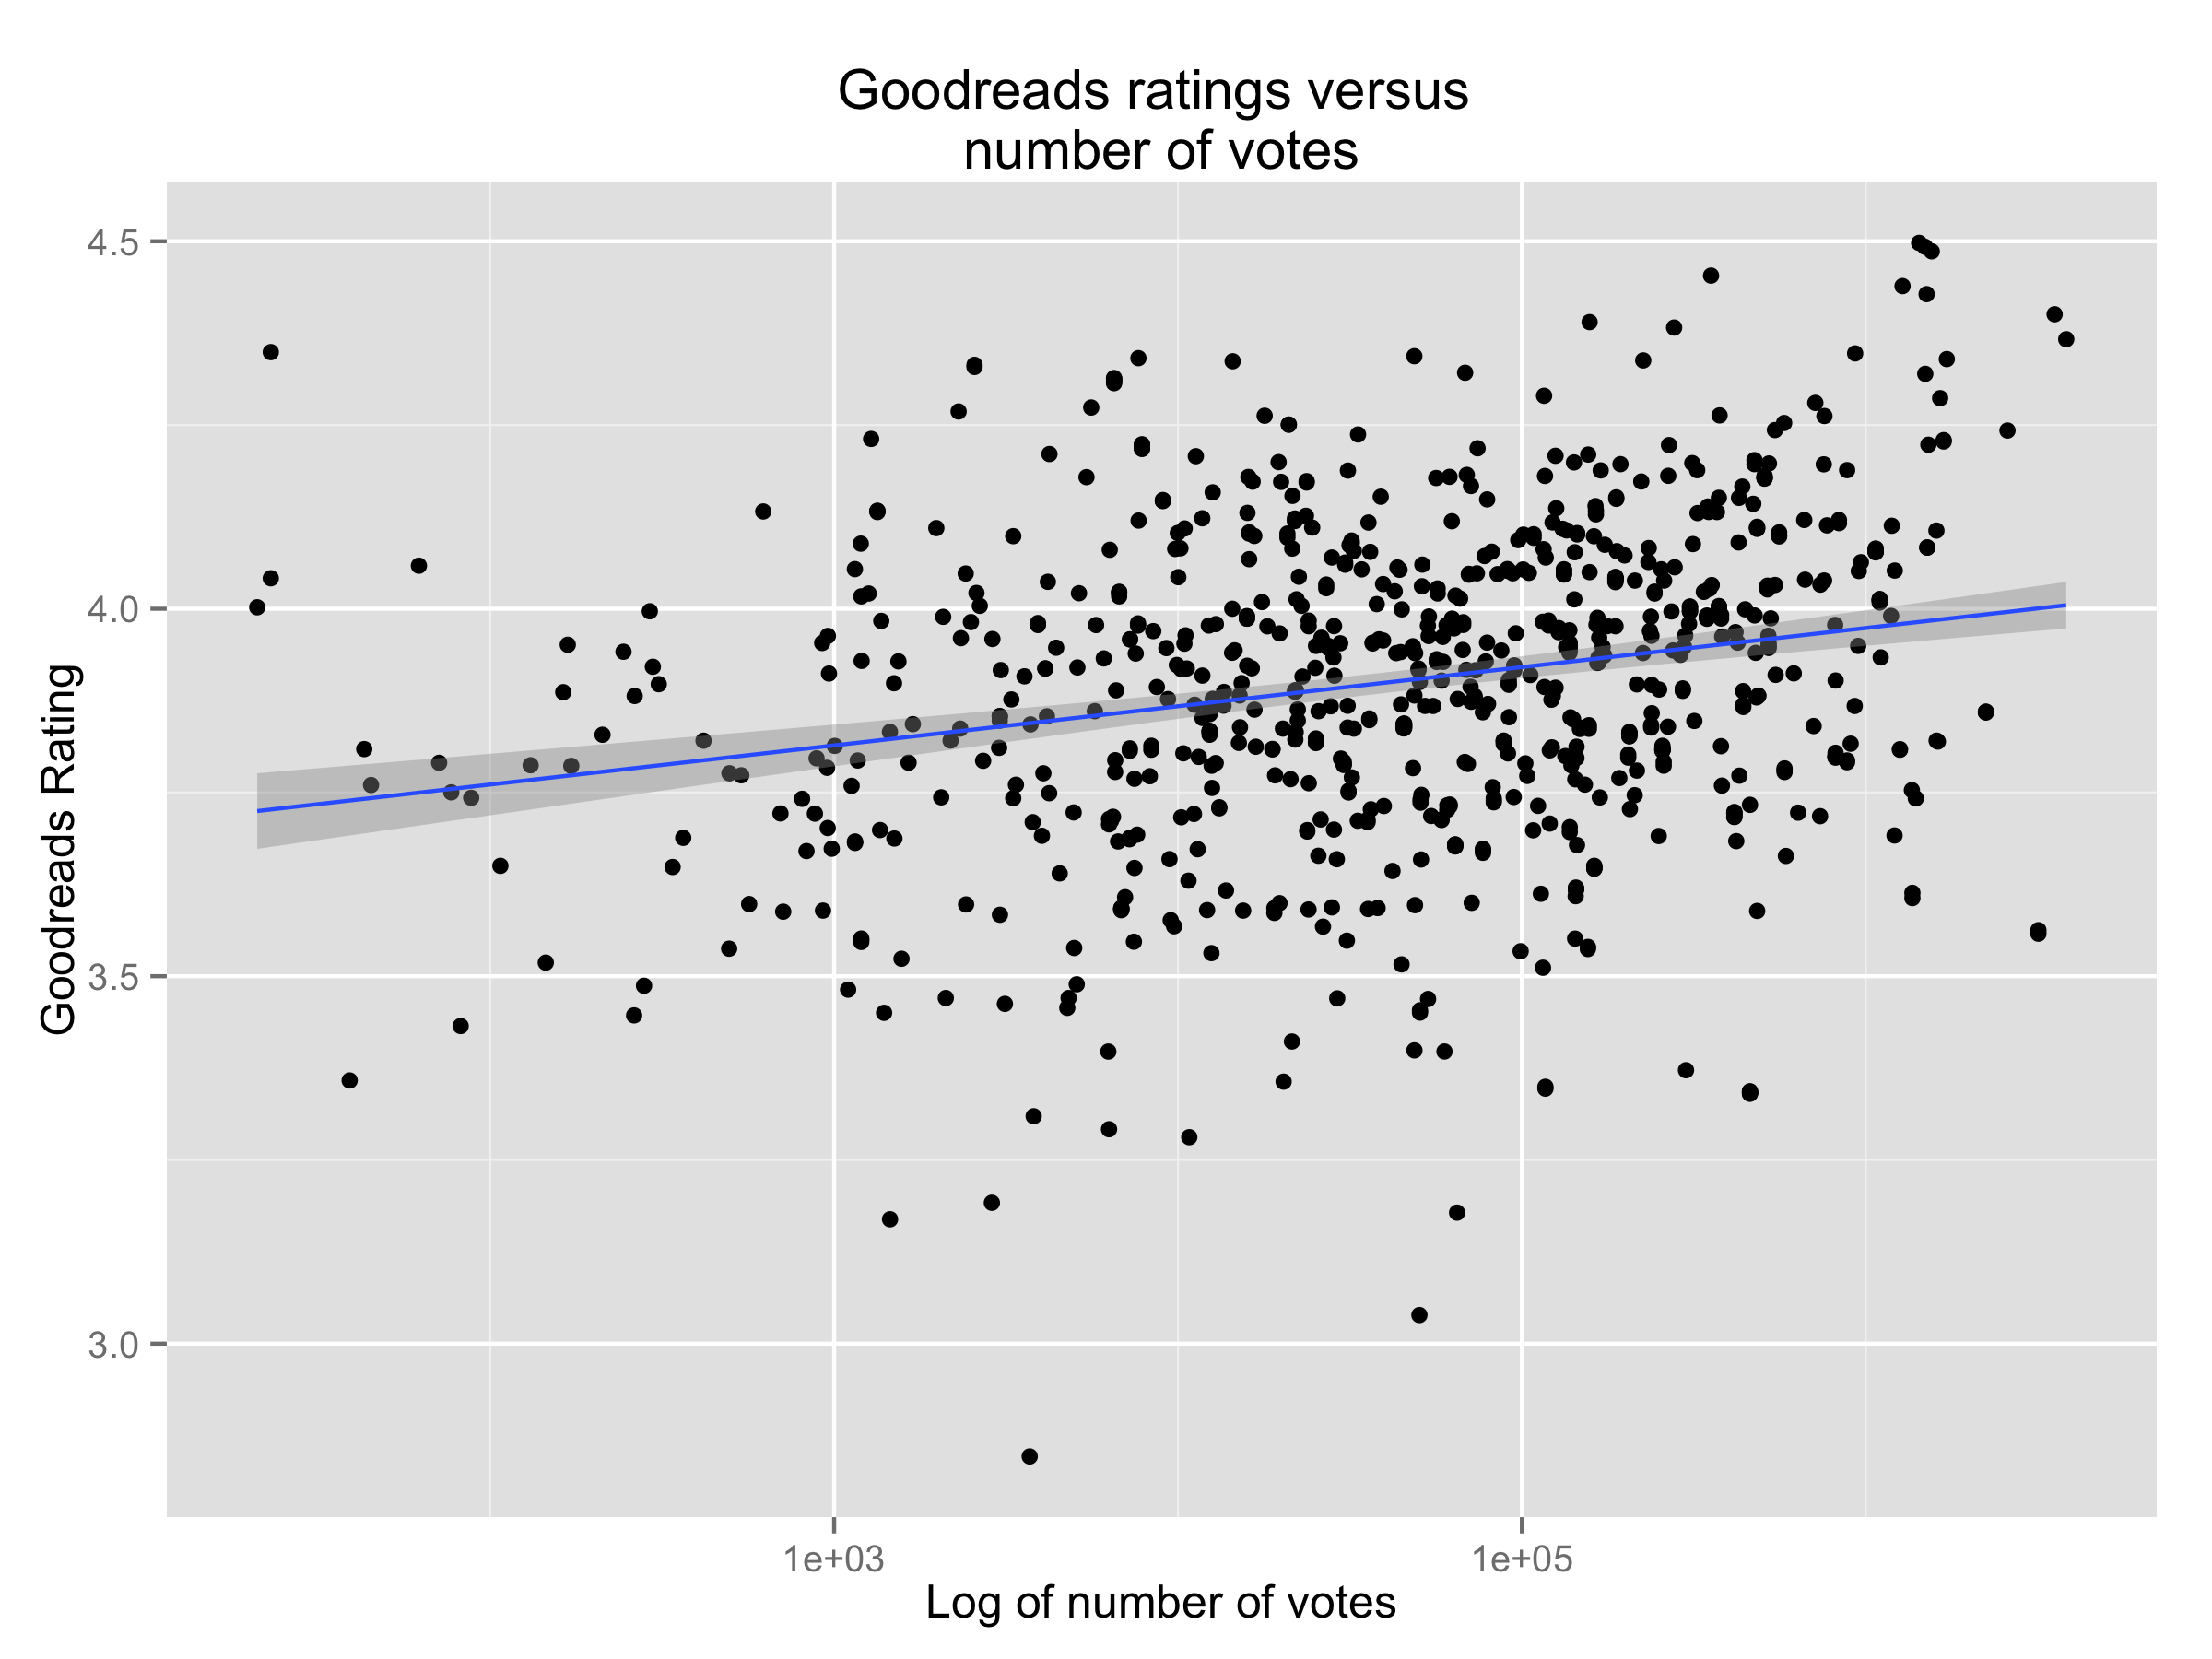
\includegraphics[scale=0.1]{ratingsbooks}
    \caption{Goodreads}
    \label{fig:1a}
  \end{subfigure}%
  \begin{subfigure}[b]{.5\linewidth}
    \centering
    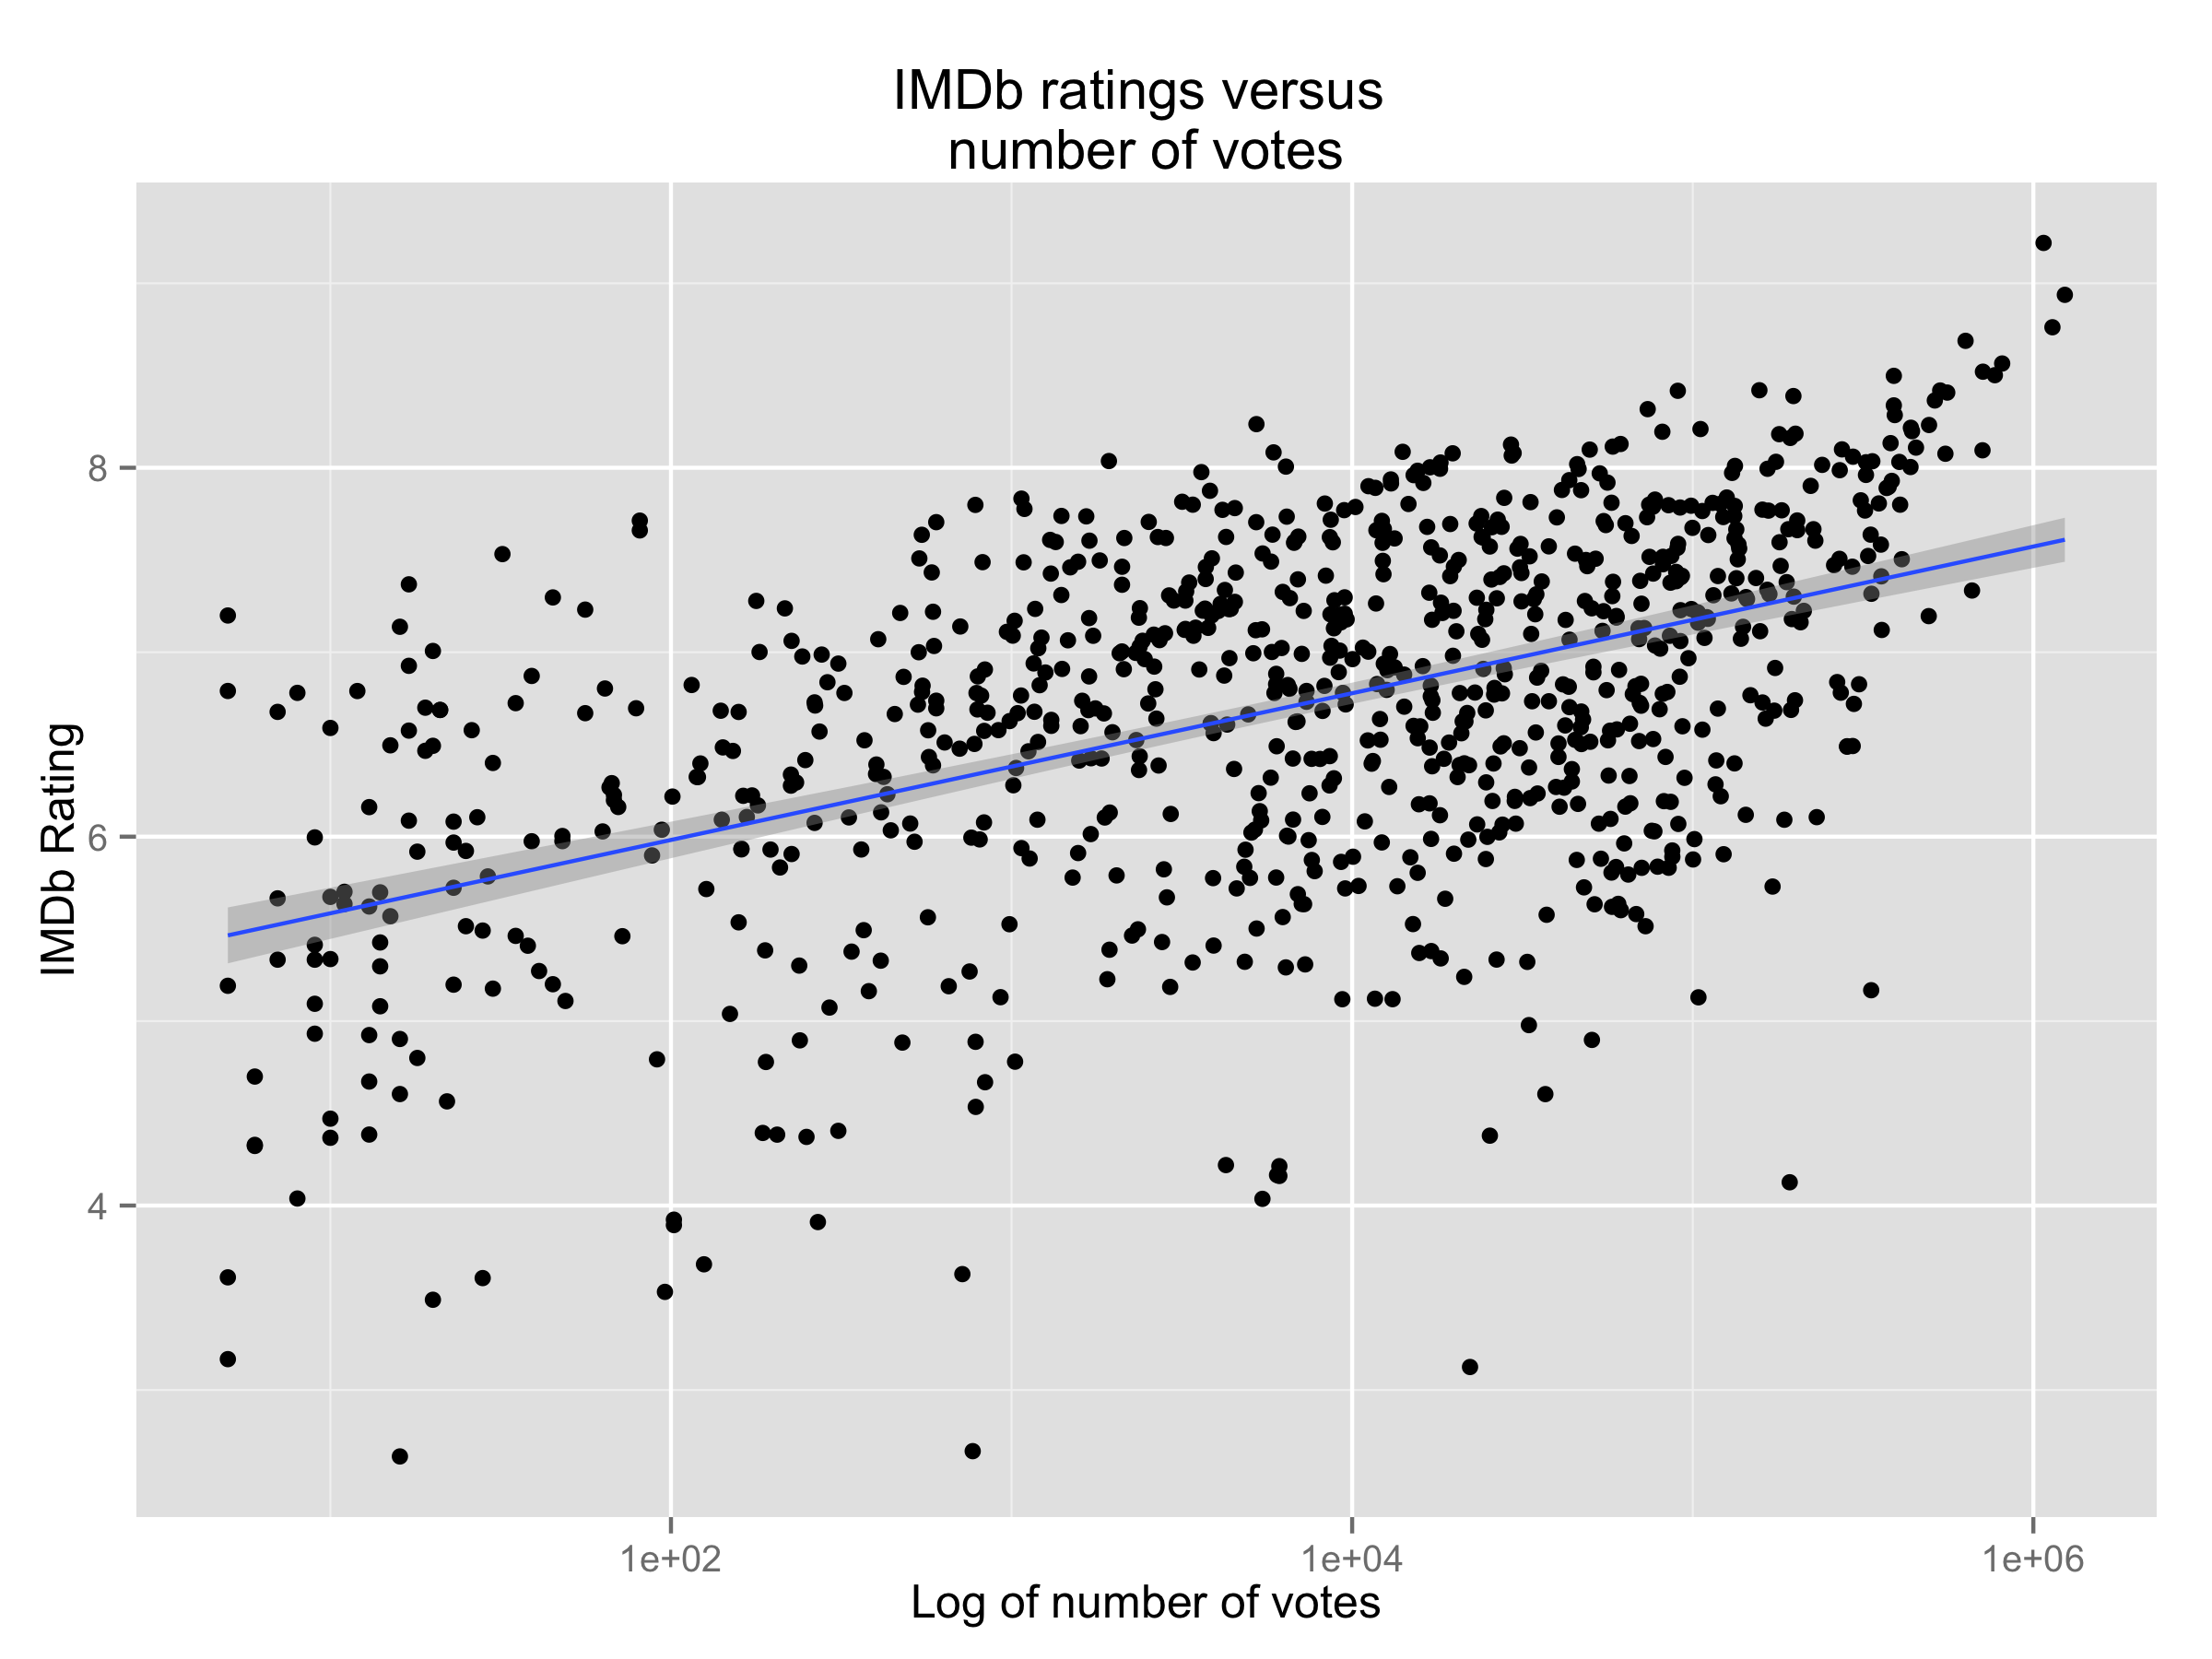
\includegraphics[scale=0.1]{ratingsimdb}
    \subcaption{IMDb}
    \label{fig:1b}
  \end{subfigure}
  \caption{Avereage rating compared to number of votes cast. We see an upwards trend in both}
  \label{fig:1}
\end{figure}

In their seperate listing of top 250 movies, IMDb uses a so-called Bayesian average in ratings, taking into account the number of votes given. It is calculated as:
$$WR (\text{Weighted Ranking})=\frac{v}{v+m}R+\frac{m}{v+m}C$$
Where $R$ is the average rating for the movie, $v$ is the number of votes for the movie, $m$ is a minimum number required to be listed on the top 250 and $C$ is the mean rating for the report. 

We have considered using a Bayesian average in the model of IMDb in calculating average rated, as we have the data needed to do so. However, we stick to the original ratings. Under the Bayesian average, any rating with a number of votes given under an arbitrary number ie. 1000, will converge to the mean rating, and pull the ratings above the arbitrary number towards the mean in decreasing degree with the number of votes cast. This will give the figures in figure \ref{fig:1} a trumpet-like shape and give a large number of ratings the mean rating, destroying the ordinality that we are trying to examine. 

Even though the number of votes cast, intuitively should signal a greater weight or certainty about the rating, there are som biases that should be taken into account

Herding is in line with the data in figure \ref{fig:1}

Top movies are most exposed





\end{document}


